\documentclass{article}
\usepackage[utf8]{inputenc}
\usepackage{graphicx}
\graphicspath{ {/images/} }

\title{Présentation de la méthode Mérise}
\author{BRUNO Lùca, LE COZ Yann, SEA-PHANH Calvin}

\begin{document}

\maketitle

\textbf{MERISE est une méthode de conception, de développement et de réalisation de projets informatiques.} \\

\text{Le but de cette méthode est d'arriver à concevoir un système d'information. La méthode MERISE est basée sur la séparation des données et des traitements à effectuer en plusieurs modèles conceptuels et physiques.} \\

\text{La séparation des données et des traitements assure une longévité au modèle. En effet, l'agencement des données n'a pas à être souvent remanié, tandis que les traitements le sont plus fréquemment.} \\

\text{La méthode MERISE date de 1978-1979, et fait suite à une consultation nationale lancée en 1977 par le ministère de l'Industrie dans le but de choisir des sociétés de conseil en informatique afin de définir une méthode de conception de systèmes d'information. Les deux principales sociétés ayant mis au point cette méthode sont le CTI (Centre Technique d'Informatique) chargé de gérer le projet, et le CETE (Centre d'Etudes Techniques de l'Equipement) implanté à Aix-en-Provence. }\\

\textbf{Cycle d'abstraction de conception des systèmes d'information}\\

\text{La conception du système d'information se fait par étapes, afin d'aboutir à un système d'information fonctionnel reflétant une réalité physique. Il s'agit donc de valider une à une chacune des étapes en prenant en compte les résultats de la phase précédente. D'autre part, les données étant séparées des traitements, il faut vérifier 
la concordance entre données et traitements afin de vérifier que toutes les données nécessaires aux traitements sont présentes et qu'il n'y a pas de données superflues.} \\

\text{Cette succession d'étapes est appelée cycle d'abstraction pour la conception des systèmes 
d'information : }\\


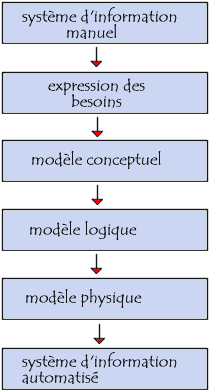
\includegraphics[scale=1.5]{merise} \\

\text{L'expression des besoins est une étape consistant à définir ce que l'on attend du système d'information automatisé, il faut pour cela :} \\

\begin{itemize}
    \item faire l'inventaire des éléments nécessaires au système d'information
    \item délimiter le système en s'informant auprès des futurs utilisateurs 
\end{itemize}
 
 \text{Cela va permettre de créer le MCC (Modèle conceptuel de la communication) qui définit les flux d'informations à prendre en compte. } \\
 
 \text{L'étape suivante consiste à mettre au point le MCD (Modèle conceptuel des données) et le MCT (Modèle conceptuel des traitements) décrivant les règles et les contraintes à prendre en compte.} \\
 
 \text{Le modèle organisationnel consiste à définir le MOT (Modèle organisationnel des traitements) décrivant les contraintes dues à l'environnement (organisationnel, spatial et temporel).}

\end{document}
